\section{Sprint 5}%Autenticación
\subsection{Planificación}

	\textbf{Inicio: } 10 de Septiembre del 2015
	
	\textbf{Fin:} 27 de Septiembre del 2015 



\subsection{Descripción}

Este sprint tiene por objetivo definir un proceso de autenticación del usuario para con la API, sin importar el perfil del mismo, que garantice un nivel de seguridad adecuado para tranquilidad en el uso de la aplicación por parte de los interesados. 

\subsection{User Stories relacionados}
La \textbf{Tabla \ref{US-Sprint5} } indicará las características de cada user story para guiarnos en el desarrollo del sprint.
\begin{comment}
	como usuario quiero contar con un acceso único y privado a mi información. Agregaría este user story, habría que ver la traza con el documento de diseño para que queden balanceados.
\end{comment}
\begin{table}[h]
    \label{US-Sprint5}
	%\resizebox{\textwidth}{!}{
    \centering
	\begin{tabular}{|l|p{9cm}|}
	\hline
        \multicolumn{1}{|c|}{\textbf{ID}} &
        \multicolumn{1}{|c|}{\textbf{Enunciado de la historia}} \\          
    \hline
        \textbf{US-\ref{modificarPermisos}} & Como paciente, quiero modificar los permisos de visualización de mis datos con respecto a cada uno de los integrantes de grupo familiar para tener un control total sobre mi privacidad. \\
     \hline 
        \textbf{US-\ref{validarUsuario} } & Como usuario quiero contar con un acceso único y privado a mi información. \\
     \hline 
     
    \end{tabular}
%     }

\end{table}
\subsection{Modelo de datos}
El Diagrama propio de este sprint se puede ver en la \textbf{Figura \ref{5-clase_autenticacion}}, allí se indican exactamente las clases que se usarán en este sprint y que serán detalladas con detenimiento en el presente documento. 

\begin{figure}[h]
        \centering
        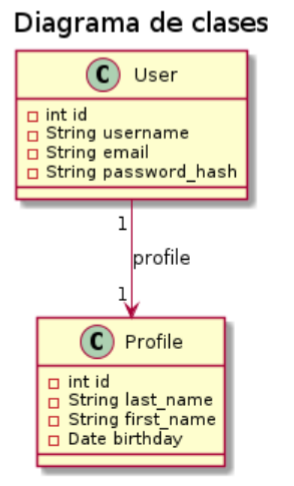
\includegraphics[width=0.3\textwidth]{img/clases_auth}
        \caption{Diagrama de clases autenticación.}
		\label{5-clase_autenticacion}
    \end{figure}

\subsection{Modelo funcional} 
Se define el diagrama de casos de uso del presente Sprint \textbf{[Figura \ref{4-cu_autenticacion}]}.

    \begin{figure}[h]
        \centering
        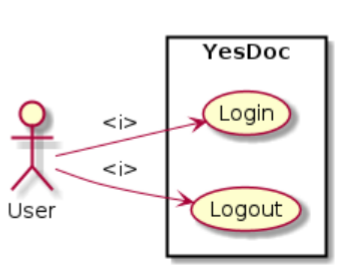
\includegraphics[width=0.4\textwidth]{img/cu_autenticacion}
        \caption{Casos de uso autenticación}
		\label{4-cu_autenticacion}
    \end{figure}

	{\scriptsize
	\begin{center} %sidewaystable
	\centering
	%\begin{adjustbox}{max width=\textheight}
    \resizebox{\textwidth}{!}{
		\begin{tabular}{|l|l|l|p{5cm}|l|p{1cm}|}
			\hline
			\textbf{Area a cargo} &
			\textbf{Responsable} &        
			\textbf{Revisor} &        	        
			\textbf{Tarea} &
			\textbf{US} &
			\textbf{Tiempo dedicado} \\
			\hline
			
	    Backend& Michael Manganiello& Franco Canizo & Generación del modelo User y relación del mismo con el modelo Profile.  & US-\ref{modificarPermisos} \& US-\ref{validarUsuario} & 13hs
	     \\ \hline
	    Backend& Michael Manganiello& Franco Canizo & Generación del recurso relacionado con el modelo User y los métodos post y get que manejan los operadores HTTP correspondientes.  & US-\ref{modificarPermisos} \& US-\ref{validarUsuario} & 11hs
	    \\ \hline
	    Backend& Michael Manganiello & Franco Canizo& Generación del recurso para obtener un token para un usuario autenticado.  & US-\ref{modificarPermisos} \& US-\ref{validarUsuario} &9hs
	    \\ \hline
		Backend& Michael Manganiello & Franco Canizo& Se creó el recurso /my/profile, que hace uso de la autenticación para obtener la información del perfil asociado al usuario. Permite los métodos GET y PUT. & US-\ref{modificarPermisos} \& US-\ref{validarUsuario} & 4hs
		\\ \hline
		Backend& Michael Manganiello & Franco Canizo& Se crearon dos nuevos recursos GET:
		\begin{itemize}
			\item 		/my/measurements
			\item		/my/measurements/latest
		\end{itemize}
		Ambos recursos requieren autenticación (ya sea mediante usuario y contraseña, o token de sesión) y retornan las mediciones asociadas al perfil del usuario autenticado. Por lo tanto, no es necesario especificar un id de perfil, sino que se toma el perfil del usuario que realiza la petición. & US-\ref{modificarPermisos} \& US-\ref{validarUsuario} & 8hs
		\\ \hline
		Frontend& Yanina Morales  & Ivan Terreno& Se cambiaron las referencias a los recursos para utilizar los que requieren que el usuario se encuentre logueado & US-\ref{modificarPermisos} \& US-\ref{validarUsuario} & 12hs
		\\ \hline
		Frontend& Yanina Morales  & Ivan Terreno& Se corrigieron errores para que el navbar sea responsive & US-\ref{modificarPermisos} \& US-\ref{validarUsuario} & 8hs
		\\ \hline		
	    \end{tabular}
        }
	    %\end{adjustbox}
    	\end{center}
	}
    
\subsubsection{Definición de modelos}
La definición del modelo User es bastante compleja ya que define métodos para tomar la password  y guardarla como un hash, a su vez, puede recibir passwords encriptadas y desencriptarlas. Por otro lado, define métodos para la generación y verificación del token asignado al usuario. Por último, define una relación uno a uno con el modelo Profile.

\subsubsection{Recursos}
El desafío en cuanto a la definición de recursos radica en que según lo que establece REST, la restricción de que la API debe ser stateless invalida la posibilidad de usar sesiones para que la API sea escalable, es por esto que definimos una solución que se presenta en un punto gris entre puristas de REST y quienes realmente no hacen REST. La solución consiste en generar un token para el usuario autenticado el cual se almacena en las cookies y es usado en cada solicitud para autenticar al usuario. Por esto se definen recursos para dar de alta al usuario y para entregarle un token.

	\begin{lstlisting}[language=Python]
	api.add_resource(UserView, '/users/<int:id>')
	api.add_resource(UserList, '/users')
	api.add_resource(Token, '/token')
	api.add_resource(MyUserView, '/my/user')
	\end{lstlisting}

\subsection {Salidas del Sistema}

\begin{enumerate}
	\item \textbf{Solicitud post al recurso del perfil}
    
	Para crear un usuario debe existir un perfil creado, para esto usamos el recurso ``\/profiles'' a través del método POST y pasando como argumento los datos first\_name, last\_name, birthday y gender\_id.
    \item \textbf{Solicitud post al recurso del user}
    
    Realizamos ahora una solicitud HTTP, con método post utilizando curl al recurso del usuario usando el id del perfil creado previamente:

\begin{verbatim}
curl -i http://localhost:5000/users -H "Content-Type: 
application/json" -X POST -d '{"username":"akathy", 
"email":"kathy@gmail.com", "password":"kathy1234", 
"profile_id":"2"}'
\end{verbatim}
    
    Obtenemos la siguiente respuesta de la API, con un código 201.
    
\begin{lstlisting}[language=json]
HTTP/1.0 201 CREATED
Content-Type: application/json
Content-Length: 425
Server: Werkzeug/0.10.4 Python/2.7.6
Date: Tue, 20 Oct 2015 05:21:37 GMT

{
    "resource": {
        "email": "kathy@gmail.com", 
        "id": 2, 
        "profile": {
            "birthday": "1989-06-17", 
            "first_name": "Katherina", 
            "gender": {
                "description": "female gender", 
                "id": 2, 
                "name": "female"
            }, 
            "id": 2, 
            "last_name": "Aguirre"
        }, 
        "username": "akathy"
    }
}
\end{lstlisting}

    \item \textbf{Solicitud post al recurso token usando user y password}
    
    Luego con este usuario y contraseña solicitamos un token al recurso correspondiente:

\begin{verbatim}
curl -u akathy:kathy1234 http://localhost:5000/token
\end{verbatim}
   
   Obtenemos así el token que debe ser almacenado en las cookies, tendrá una duración de 10 minutos y será utilizado en cada solicitud para autenticación.
   
\begin{lstlisting}[language=json]
{
    "resource": {
        "duration": 600, 
        "token": "eyJhbGciOiJIUzI1NiIsImV4cCI6MTQ0NTMxOTM3MCwiaWF0IjoxNDQ1MzE4NzcwfQ.eyJpZCI6Mn0.2eZRjbMq9tg4GykJx8EU-Ux4ZoyUW6WnBlADsvnpQvE"
    }
}
\end{lstlisting}

\end{enumerate}

\clearpage
\subsection{Criterios de aceptación}

\begin{center}
\begin{longtable}{|p{0.5cm}|p{4cm}|p{4cm}|p{5cm}|}
\hline \hline \rowcolor[gray]{0.9}
	\multicolumn{4}{||c|}{\textbf{Criterio de aceptación}} \\
    \hline  \rowcolor[gray]{0.9}
        \textbf{Id} &
        \textbf{Contexto} &
        \textbf{Evento}&
        \textbf{Resultado} \\
    \hline
1&En caso de que exista un usuario registrado con el mismo username & al ejecutar el método post del recurso \/users  & El sistema devolverá un json vacío y un código de error 400 \\ \hline
	\hline
2&En caso de que exista al menos un usuario registrado & al ejecutar el método get del recurso \/users  & El sistema devolverá una lista de json con los datos de los users registrados \\ 		\hline
	\hline
3&En caso de que exista un usuario registrado con el mismo username & al ejecutar el método post del recurso \/users  & El sistema devolverá un json vacío y un código de error 400 \\ \hline
    \hline
4&En caso de que no exista un usuario registrado con el id indicado & al ejecutar el método get\/put del recurso \/users\/id  & El sistema devolverá un json con un mensaje de error y un código de error 404 \\ \hline

  \end{longtable}
\end{center}

\begin{comment}
	Cuando devolvería 401 el recurso del token.
\end{comment}

\subsection{Casos de prueba}

\subsubsection{Pruebas de integración entre módulos del Sistema}

\subsubsection{Pruebas de carga}

\subsubsection{Pruebas de seguridad por niveles de usuarios}


\subsection{Pruebas ejecutadas}
Aqui se realizará una conclusión general de lo que se descubrió en las pruebas.
        %
	\begin{itemize}
		\item \textbf{¿Que fue bien?}
        	\begin{itemize}
				\item        Las cargas y ediciones se llevan a cabo correctamente.
			\end{itemize}

   		\item \textbf{¿Que se mejoró?}
        	\begin{itemize}
                \item \textbf{Cerrado} problema
			\end{itemize}

   		\item \textbf{¿Que se puede mejorar?}
        	\begin{itemize}
		        \item \textbf{Abierto} En el futuro se deberá mejorar ...
            \end{itemize}
        

	\end{itemize}